\chapter{Theoretical Background}
\label{ch:theory}

\section{Standard Model}
\label{sec:standard_model}

Developed throughout the 1960s and 1970s, the Standard Model provides the most complete description of observable matter in the universe to date.
It is a classification of all confirmed subatomic particles currently known, and predicts the most accurate results of any scientific theory ever measured.
Each of the electromagnetic, weak, and strong fundamental forces are well described by this formulation.
These three are described by an $\SUthree \times \SUtwo \times \Uone$ group, where the $\SUthree$ corresponds to the strong force, the $\SUtwo$ corresponds to the weak force, and the $\Uone$ corresponds to the electromagnetic force.
The remaining fundamental force, gravity, is not included in the Standard Model.
It is negligible on the scale of the masses of fundamental particles, and will be ignored in the discussions that follow.


\subsection{Electromagnetic Force}
\label{ssec:electromagnetic}

The electromagnetic force is responsible for the forces between objects with electric charge, most notably binding together electrons and protons to form atoms and the structures they comprise.
The theory of electromagnetic interactions is known as Quantum Electrodynamics (QED).
Within this theory, the mediator of this force is the photon, a massless vector boson.
As there is only a single mediator, and a single conserved quantity (electric charge), the formulation of QED is relatively simple compared to the other forces.
Still, the predictions it makes show astounding consistency with experiment, such as correctly calculating the anomalous magnetic dipole moment of the electron to more than 10 significant figures.
Much of this success is due to QED being calculable through perturbation theory, where corrections are applied in terms of higher order factors of the coupling constant, $\alphaQED$.
This is possible due to its relatively small value ($\alphaQED \approx 1/137$), as the terms are convergent below very high orders of $\alphaQED$. 

\subsection{Weak Force}
\label{ssec:weak}

The weak force is responsible for radioactive decay and other subatomic phenomena.
This is distinct from the electromagnetic and strong interactions, where the constituent particles cannot change their types (or flavors).
The mediators of this force are the $\W$ and $\Z$, which are massive vector bosons.
Not only are each of their masses non-zero, they are extremely heavy particles at \SIlist{80.4;90.2}{\GeV}, respectively \cite{ref:Olive:2014}.
The unit of energy, \si{\eV}, represents the amount of energy required to move a charge of $e$ through a potential difference of \SI{1}{\volt}.
These large masses not only limit the interaction distance of the weak force, but also minimize the interaction strength (which is inversely proportion to mass).
Furthermore, the large $\W$ and $\Z$ masses also lead to much slower interaction times, further reducing the effects of the weak force in comparison to the strong and electromagnetic forces.


In addition to transforming particle flavor, the weak force is also unique in its violation of various symmetries.
The first discovery of symmetry violation came in 1957, when Wu and others \cite{ref:Wu:1957} discovered the weak force did not behave identically under parity ($\sP$) transformations (i.e., mirror reflection).
To account for this, a new theory conserving a compound symmetry was proposed.
This combined charge conjugation ($\sC$), the swapping of particles with their antiparticles, with parity to form $\sCP$ parity.
However, in 1964, evidence of $\sCP$ violation was also discovered by Cronin and Fitch \cite{ref:Christenson:1964}.
The resolution to this symmetry conservation involves yet a third symmetry, time reversal ($\sT$), in which time is replaced with its negative ($t \rightarrow -t$).
While the weak force violates these symmetries individually, the application of all three ($\sCPT$) is conserved across all known processes, and is known as the $\sCPT$ Theorem.


At higher energy scales, the electromagnetic and weak forces unify into the electroweak force.
In this theory, there are initially four massless gauge bosons mediating the interactions.
As a result of the Higgs mechanism, the initial gauge symmetry is broken at lower energies, and three of these bosons acquire a mass.
These three bosons are the $\W^\pm$ and $\Z$, while the remaining massless boson is the $\photon$.
The energies scales required for this unification were only present in the early universe.
Before this, it is also believed there was an epoch of even higher energy, in which the electroweak force merged with the strong force.


\subsection{Strong Force}
\label{ssec:strong}

The strong force is responsible for binding together particles known as hadrons.
The theory of strong interactions is known as Quantum Chromodynamics (QCD).
Like the electromagnetic force, the mediator of the strong force is also a massless vector boson, the gluon.
However, while massless particles typically correspond to an infinite interaction range, the strong potential becomes very large at higher separations.
This prevents the most fundamental particles which interact through the strong force, known as quarks (see \Cref{sssec:fermions}), from existing as isolated entities in a process known as confinement.
The typical interaction range is on the order of the proton radius, around \SI{e-15}{\m}.
QCD calculations face serious challenges, however, as the coupling constant is not small ($\alphaQCD \gtrsim 1$).
This excludes the use of perturbation theory for most cases, as the higher order terms do not converge.


Strong interactions are associated with a corresponding conserved quantity known as the color charge. 
Despite its name, however, the term 'color' has no association with light, which is a purely electromagnetic phenomena.
There are three colors associated with this charge, red ($\cRed$), green ($\cGreen$), and blue ($\cBlue$).
For anti-particles, there are oppositely charged values ($\acRed, \acGreen,$ and $\acBlue$).
In order for hadrons to be formed, the total color values of the constituents must be colorless.
This means the total sum must involve all three colors ($\cRed \cGreen \cBlue$ or $\acRed \acGreen \acBlue$) or pairs of opposite colors ($\cRed \acRed, \cGreen \acGreen, $ or $\cBlue \acBlue$).
However, these individual colors are not observable in nature.
Because particles with different color values are distinct, this effectively triples the number of possible particle combinations, due to combinatorics.


Unlike the photon, which does not carry an electric charge, gluons do possess a color charge.
There are eight possible color combinations which a gluon may possess, which are typically expressed using the Gell-Mann representation of $\SUthree$.
With this basis, each gluon is linearly independent, and no combination of gluons can be used to form a color singlet state.
This non-zero charge of the force carrier makes QCD significantly more complex than QED.
In fact, carrying color charge means gluons can also interact with each other directly, leading to certain theoretical states such as glueballs. 


\subsection{Elementary Particles}
\label{ssec:elementary_particles}

There are two primary groups contained in the Standard Model, fermions and bosons. 
This division is based on the Spin Statistics theorem, where fermions (bosons) have half-integer (integer) spins.
As described by the Pauli Exclusion principle, nature restricts fermions from occupying the same quantum state.
Bosons, however, do not have this restriction, and can have any number occupying the same state.

\begin{figure}[H]
\centering
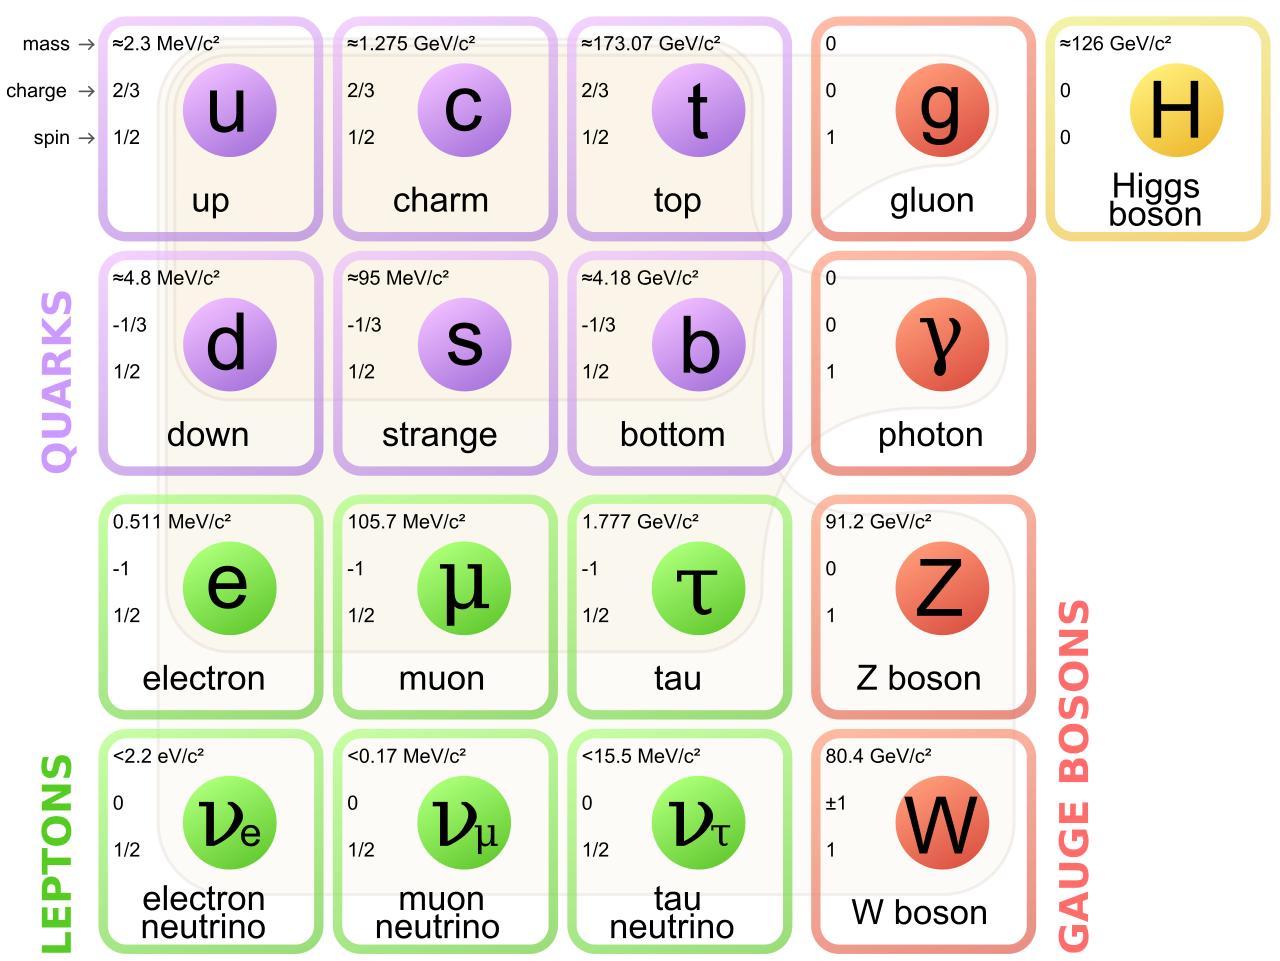
\includegraphics[scale=0.30]{figures/images/standard_model.png}
\caption{The standard model of particle physics.}
{It is comprised of two main groups: fermions, which includes the quarks and leptons, and bosons, which includes the gauge bosons and the Higgs boson. Image reproduced courtesy of \cite{ref:Wikimedia:2006}. }
\label{fig:standard_model}
\end{figure}


\subsubsection{Fermions}
\label{sssec:fermions}

The fermions are divided by their interaction types into two major groups, quarks ($\quark$) and leptons ($\lepton$).
Each of these groups contains six particles with their corresponding antiparticles.
These can be grouped into three generations, which aligns particles with the same electric charges, but greatly differing masses.  
As an example, the up ($\qup$), charm ($\qcharm$), and top ($\qtop$) quarks all have an electric charge of +2/3 (in terms of the electron charge, $e$), but $\qtop$ is approximately five orders of magnitude more massive than $\qup$.
For the quarks and fermions in \Cref{fig:standard_model}, rows indicate particles with the same electric charge, while columns represent each generation of particles.


While all fundamental fermions interact weakly, and all charged fermions interact electromagnetically, only the quarks interact strongly.
Because of confinement, quarks cannot exist as isolated particles, and are only found in nature as groups of particles called hadrons.
The most common types of hadrons exist as quark-antiquark pairs, known as mesons, or as groups of three quarks (or antiquarks), known as baryons.
There are, however, indications of more exotic combinations of quarks, such as tetra- ($\quark\quark\aquark\aquark$) or penta-quark ($\quark\quark\quark\quark\aquark$) states seen by recent experiments \cite{ref:Ablikim:2013,ref:Liu:2013,ref:Aaij:2015}.


While the negatively charged quarks ($\qdown, \qstrange$, and $\qbottom$) are labeled as definite states, the quarks are actually mixed states.
Through weak interactions, each of these quarks can transform into other quarks.
The probabilities for these transformations are expressed by the Cabibbo-Kobayashi-Maskawa (CKM) Matrix \cite{ref:Kobayashi:1973}, shown in \Cref{fig:ckm_matrix}.
From the experimentally measured values \cite{ref:Olive:2014}, it is evident the matrix is nearly diagonal.
It is also clear that correlations are strongest within each generation, as the off-diagonal terms are generally smaller than the diagonal ones.
Additionally, though the convention splits the negatively charged quarks into mixed states (leaving the positively charged quarks fixed), this choice has no physical basis.
The reverse choice of having mixed positively charged quarks is equivalent.

\begin{figure}[H]
\centering
$
\begin{bmatrix}
   |V_{ud}| & |V_{us}| & |V_{ub}| \\
   |V_{cd}| & |V_{cs}| & |V_{cb}| \\
   |V_{td}| & |V_{ts}| & |V_{tb}| \\
\end{bmatrix}
=
\begin{bmatrix}
    0.97427 \pm 0.00014 & 0.22536 \pm 0.00061 & 0.00355 \pm 0.00015 \\
    0.22522 \pm 0.00061 & 0.97343 \pm 0.00015 & 0.0414  \pm 0.0012  \\
    0.00886^{+0.00033}_{-0.00032} & 0.0405^{+0.0011}_{-0.0012} & 0.99914 \pm 0.00005 \\
\end{bmatrix}
$
\caption{The Cabibbo-Kobayashi-Maskawa (CKM) Matrix.}
\label{fig:ckm_matrix}
\end{figure}

The values of the CKM matrix are typically parameterized using three Euler angles ($\theta_{12}, \theta_{23}, \theta_{13}$) and a $\sCP$-violating phase parameter ($\delta_{13}$), where the indices represent the three generations of quarks.
This formulation allows the matrix to be cast in the ``standard'' parametrization, shown in \Cref{fig:ckm_standard}.
The form with three separated matrices clearly shows the connections between the generations of quarks.
Namely, the third shows the original formulation in terms of a single rotation, the Cabbibo angle ($\theta_{12}$).
This theory is known as the Glashow-Iliopoulos-Maiani (GIM) mechanism [\cite{ref:Glashow:1970} and was used to explain the suppression of flavor-changing neutral currents (FCNC) before the discovery of the charm quark.
% Current measurements for the standard parameters are $\theta_{12} = \ang{13.04 \pm 0.05}, \; \theta_{13} = \ang{0.201 \pm 0.011}, \; \theta_{23} = \ang{2.38 \pm 0.06}$ and $\delta_{13} = \SI{1.20 \pm 0.08}{\rad}$.

\begin{figure}[H]
\centering
$
    \begin{bmatrix}
        1 &  0      & 0      \\
        0 &  c_{23} & s_{23} \\
        0 & -s_{23} & c_{23} \\
    \end{bmatrix}
    \begin{bmatrix}
         c_{13}                  & 0 & s_{13} e^{-i\delta_{13}}  \\
         0                       & 1 & 0                         \\
        -s_{13} e^{i\delta_{13}} & 0 & c_{13}                    \\
    \end{bmatrix}
    \begin{bmatrix}
         c_{12} & s_{12} & 0 \\
        -s_{12} & c_{12} & 0 \\
         0      & 0      & 1 \\
    \end{bmatrix}
\linebreak
=
    \begin{bmatrix}
          c_{12} c_{13} 
       &  s_{12} c_{13}
       &  s_{13} e^{-i\delta_{13}} \\
         -s_{12} c_{23} - c_{12} s_{23} s_{13} e^{i\delta_{13}}
       &  c_{12} c_{23} - s_{12} s_{23} s_{13} e^{i\delta_{13}}
       &  s_{23} c_{13} \\
          s_{12} s_{23} - c_{12} c_{23} s_{13} e^{i\delta_{13}}
       & -c_{12} s_{23} - s_{12} c_{23} s_{13} e^{i\delta_{13}}
       &  c_{23} c_{13} \\
    \end{bmatrix}
$
\caption{The standard form of the Cabibbo-Kobayashi-Maskawa (CKM) Matrix.}
    {The parameterization is in terms of three angles ($\theta_{12}, \theta_{23}, \theta_{13}$) and a phase angle ($\delta_{13}$). Here, $c_{ij} = \cos\theta_{ij}$ and $s_{ij} = \sin\theta_{ij}$.} 
\label{fig:ckm_standard}
\end{figure}

The leptons are also organized into generations consisting of particles with two distinct charges.
The electron ($\lel$), muon ($\lmu$), and tau ($\ltau$) are all negatively charged particles.
There is also a neutral particle, a neutrino ($\neutrino$), corresponding to each of the charged leptons ($\vel, \vmu, \vtau$).
These are very small mass ($< \SI{1}{\eV}$) particles with extremely low interactions.
With the exception of mass, the interaction properties of each flavor are very similar.
However, the three flavors themselves are treated as separate conserved quantities.


The Standard Model assumes neutrinos to be massless particles.
However, this was violated by the discovery of neutrino oscillations, where transformations occur between neutrino flavor states due to differences in their masses.
As with the quarks, the flavor states, $\vel, \vmu$, and $\vtau$, are not the states observed in nature.
Rather, the states with definite mass, labeled $\nu_1, \nu_2,$ and $\nu_3$, are linear combinations of the three flavor states.
This can be expressed in a rotation of bases called the Pontecorvo-Maki-Nakagawa-Sakata (PMNS) matrix \cite{ref:Pontecorvo:1957,ref:Maki:1962}.
Its formulation is analogous to the CKM Matrix for quarks. 


\subsubsection{Bosons}
\label{sssec:bosons}

For each of the three forces included in the Standard Model, there are accompanying gauge bosons.  
These are the photon ($\photon$) for electromagnetic force, the $\W^\pm$ and $\Z$ for the weak force, and the gluon ($\gluon$) for the strong force.
Each of the gauge bosons is a spin-1 vector boson, which means there are three available polarization states (-1, 0, +1).  
However, since the photon and gluon are both massive, gauge invariance requires these to have transverse polarizations.
This means the spin-0 state is eliminated, and there are only two polarization states for each.
There is also the Higgs boson ($\Higgs$), which unifies the electromagnetic and weak forces, and whose interactions with other particles are responsible for their mass.
This is the only known fundamental spin-0 particle, which means it has only one polarization state.


Even with the amazing success of the Standard Model, the theory is not complete.  
Along with neutrino oscillations, other effects, such as dark matter and dark energy, remain major obstacles to constructing a unified theory.
Such a theory must also include gravity, but there remain significant difficulties in explaining its effects through a quantum field theory.
There also remains no conclusive explanation for various constants, such as the masses of the fundamental particles.
Still, the Standard Model remains the most precise description of the universe to date, and continues to provide the basis for much current and future experimental and theoretical work.


\section{Charmonium}

The majority of this analysis focuses on a specific group of particles known as Charmonium.
These particles are resonances formed by a $\qcharm \aqcharm$ pair, and can be treated analogously to the hydrogen atom.
Namely, there is a spectrum of various excited states in the Charmonium region, just as the spectrum of states associated with the emission lines of hydrogen.
The first three charmonium states to be discovered were the $\jpsi, \psi'$, and $\psi''$.
The $'$ and $''$ marks indicate their initial interpretations as the first and second excited states of the $\jpsi$, respectively.
In the current terminology, the $\psi'$ is denoted $\apsip$ and the $\psi''$ is denoted $\psipp$.
The numbers in parentheses represent the masses of the particles in \si{\MeV}.


An alternative labeling scheme for these states uses the quantum numbers for each particle.
This is written in the form $N^{2s+1}L_J$, where $N$ refers to the principal quantum number, $s$ refers to the total spin angular momentum of the particle, $L$ refers to the orbital angular momentum, and $J$ refers to the total angular momentum.
Here, the values of $L$ are in spectroscopic notation, where $L = 1, 2, 3, 4 \ldots$ is denoted $S, P, D, F \ldots$, and higher values follow alphabetically (excluding $J$).
As each of these states is comprised of two spin-$\half$ particles, the value of $s$ in this case can only be 0 (opposite) or 1 (aligned).
With this, the $\jpsi, \apsip$, and $\psipp$ can be denoted $1^3 S_1, \, 2^3 S_1$, and $1^3 D_1$.
The values of $n$ and $L$ are used for the alternate notation of $\psip$ representing $\apsip$.
However, the notation of $\psi(1D)$ is not used for $\psipp$ due to evidence of mixing in $\psipp$ between the $2^3 S_1$ and $1^3 D_1$ states that suggests more complicated underlying interactions \cite{ref:Rosner:2001,ref:Rosner:2004}.


In fact, while this model works well for states less massive than the $\psipp$, the predictions made above this often break down.
This likely reflects the greater complexity of states with energy values above that required to produce the open-charm $D$ mesons $\Dp (\qcharm\aqup)$ and $\DO (\qcharm\aqdown)$.
The $\DDbar$ threshold (twice the mass of the $\DO$) is just above the $\psip$ mass, and slightly below the $\psipp$ mass.
Therefore, the decay products of the two are drastically different, even while the available phase space is similar.
Example Feynman diagrams for these two states can be seen in \Cref{fig:OZI_psip,fig:OZI_psipp}.


\begin{figure}[H]
\centering
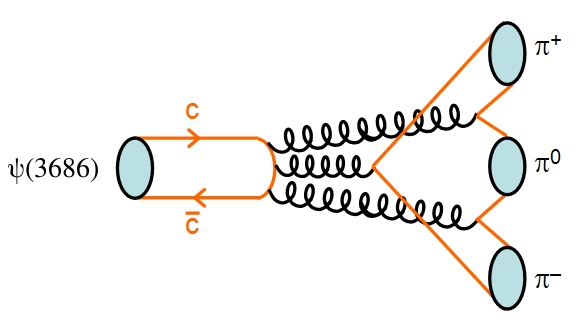
\includegraphics[scale=0.50]{figures/images/OZI_psip.png}
\caption{An example Feynman diagram for the decay of $\apsip$.}
{Without sufficient energy to produce $D$ mesons, the decays of $\apsip$ must be mediated by three hard gluons and are suppressed, as described by the OZI rule.}
\label{fig:OZI_psip}
\end{figure}

\begin{figure}[H]
\centering
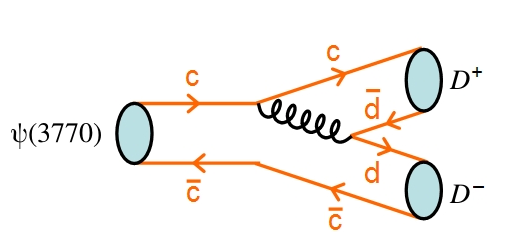
\includegraphics[scale=0.50]{figures/images/OZI_psipp.png}
\caption{An example Feynman diagram for the decay of $\psipp$.}
{With sufficient energy to produce $D$ mesons, the open-charm decays of $\psipp$ are allowed to proceed, greatly increasing the total decay width.}
\label{fig:OZI_psipp}
\end{figure}


The difference is also clearly seen in the total decay widths, where the most recent experimental averages \cite{ref:Olive:2014} are $\Gpsip = \SI{286}{\keV}$ and $\Gpsipp = \SI{27.5}{\MeV}$.
An explanation for this difference is provided by the OZI Rule, proposed independently in the 1960s by Okubo \cite{ref:Okubo:1963}, Zweig \cite{ref:Zweig:1964}, and Iizuka \cite{ref:Iizuka:1966}.
This states that any Feynman Diagram where the initial and final particles can be connected only by energetic gluons represents a suppressed decay.
In this process, the momentum transfer from the initial particles must occur entirely through these gluons, and because of the decreasing strength of the strong interaction with higher momentum transfer, the rate of these decays is inhibited.
This is further compounded by the need for three gluons in such an interaction, as one gluon could not conserve color charge, and two could not converse $\sC$-parity.
Once above the $\DDbar$ threshold, the allowed open-charm decays dominate, and the total width is greatly increased.
This dominance points to a high branching fraction expected for decays of the type $\psipptoDD$.

